\title{Relazione di ``Metodi del Calcolo Scientifico''}
\author{
	Simon Vocella \\
	Matricola: 718289
}
\date{\today}

% OK [LD] teoria
% OK [LD] jtransform
% OK [LD] i listati dei programmi
% OK [LD] risultati
% OK [LD] conclusioni

% OK [DCT2] teoria
% OK [DCT2] jtransform
% OK [DCT2] i listati dei programmi
% OK [DCT2] risultati
% OK [DCT2] conclusioni
% TODO [DCT2] leggere una o piu' immagini a scelta in toni di grigio in formato bitmap, trasformarle tramite la DCT2 e studiare cosa succede se vengono tagliate delle frequenze. Usare la versione FAST. 

\documentclass[12pt]{article}
\usepackage[margin=1.5cm]{geometry}
\usepackage[italian]{babel}
\usepackage{booktabs}
\usepackage{algorithm}% http://ctan.org/pkg/algorithm
\usepackage{algpseudocode}% http://ctan.org/pkg/algorithmicx
\usepackage{algorithmicx}
\usepackage{lipsum}% http://ctan.org/pkg/lipsum
\usepackage{float}% http://ctan.org/pkg/float
\usepackage{graphicx}
\usepackage{amsfonts}
\usepackage{amsmath}
\usepackage{listings}
\usepackage{subfigure}
\lstset{language=Java, basicstyle=\small}
\lstset{linewidth=\textwidth, showstringspaces=false}
\lstset{frame=trBL}

\begin{document}
\maketitle
\tableofcontents

\section{Lu Decomposition}
\subsection{Teoria}
Sia A una matrice invertibile. Allora A pu\`o essere decomposta come
\begin{center} $\mathbf{PA} = \mathbf{LU}$ \end{center}
dove P \`e una matrice di permutazione, L \`e una matrice triangolare inferiore a diagonale unitaria ($l_{ii} = 1, \forall i$) e U \'e una matrice triangolare superiore. \\\\
La decomposizione LU \`e simile all'algoritmo di Gauss. Nell'eliminazione gaussiana si prova a risolvere l'equazione matriciale
\begin{center} $\mathbf{A} \mathbf{x} = \mathbf{b}$ \end{center}
Il processo di eliminazione produce una matrice triangolare superiore U e trasforma il vettore b in b'
\begin{center} $\mathbf{U} \mathbf{x} = \mathbf{b}'$ \end{center}
Poich\`e U \`e una matrice triangolare superiore, questo sistema di equazioni si pu\`o risolvere facilmente tramite sostituzione all'indietro.
Durante la decomposizione LU, per\`o, b non \`e trasformata e l'equazione pu\`o essere scritta come
\begin{center} $\mathbf{A} \mathbf{x} = \mathbf{L} \mathbf{U} \mathbf{x} = \mathbf{b}$ \end{center}
cos\`i possiamo riusare la decomposizione se vogliamo risolvere lo stesso sistema per una differente b. \\\\
Nel caso pi\`u generale, nel quale la fattorizzazione della matrice comprende anche l'utilizzo di scambi di riga nella matrice, viene introdotta anche una matrice di permutazione P, ed il sistema diventa:
\begin{center} $\left\{ \begin{array}{l} Ly=Pb\\ Ux=y\end{array}\right.$ \end{center}
La risoluzione di questo sistema permette la determinazione del vettore x cercato.

\subsection{Jama}
JAMA \`e un pacchetto di algebra lineare di base scritto in Java. Fornisce le classi a livello di utente per la costruzione e la manipolazione di matrici reali, dense. \`E pensato per fornire funzionalit\`a sufficienti per problemi di routine. \\
\\
Sono disponibili cinque scomposizioni fondamentali della matrice JAMA:
\begin{itemize}
\item La decomposizione di Cholesky, matrici simmetriche definite positive
\item Decomposizione LU (eliminazione gaussiana) di matrici rettangolari (Quella che usiamo in questo caso)
\item Decomposizione QR di matrici rettangolari
\item Decomposizione autovalore di matrici quadrate e simmetriche sia nonsymmetric
\item Valore Singolare decomposizione di matrici rettangolari
\end{itemize}
Funzionalit\`a non coperte: JAMA non \`e affatto un' ambiente completo algebra lineare. Per esempio, non supporta matrici con struttura particolare o per ulteriori decomposizioni specializzati (ad esempio Shur, autovalore generalizzato). Matrici complesse non sono incluse.

\subsection{Programma lu-decomposition}
Per il progetto ho deciso di utilizzare Jama, perch\`e sembra essere veloce e semplice da implementare. Non supporta matrici i valori complessi e per questo non ho potuto calcolare gli autovalori delle matrici rand, che ho lasciato ad n.a.\\
Qui \`e listato il programma principale.

\newpage
\lstinputlisting[caption=lu-decompostion,label=lst:java]{../../lu-decomposition/src/Main.java}
\newpage

\subsection{Risultati e conclusioni}
Qui presentiamo i valori dei test precedenti con cui dovremmo confrontare i valori ottenuti.\\
Quando viene calcolato l'errore relativo e l'errore sulla prima componente, manteniamo lo stesso ordine di grandezza nella maggior parte di casi e, a volte, perdiamo o guadagniamo un ordine di grandezza nel caso di matrici bad e very bad. \\
Nel caso del calcolo del settimo autovalore i risultati sono praticamente identici. \\
Nella tabella dei valori ottenuti abbiamo aggiunto due colonne: Time to solve che \`e il tempo di calcolo della lu-decomposition e il tempo di calcolo degli autovalori. \\
Entrambi i tempi si matengono bassi tranne nel caso di rand-5000 per il tempo di calcolo della lu-decomposition e eig-5000 nel caso del calcolo dei suoi autovalori. \\

\begin{table}[h]
\caption {Valori dei test precedenti} \label{tab:title}
\begin{center}
\begin{tabular}{|l|r|r|r|}
\hline
Test         &	Errore Relativo  &	Errore Prima Comp  & Autovalore n.7 \\
\hline
     easy-10 &	    4.242156e-016 &	     6.661338e-016 &  				 7.000000 \\
    easy-100 &	    2.019904e-015 &	     3.330669e-015 &           7.000000 \\
   easy-1000 &	    2.654198e-014 &	     1.554312e-014 &           7.000000 \\
     rand-10 &	    5.607561e-015  &	   1.132427e-014 &               n.a. \\
    rand-100 &	    8.760746e-014 &	     2.065015e-014 &               n.a. \\
   rand-1000 &	     3.827585e-012 &	   5.317968e-013 &               n.a. \\
   rand-5000 &	   1.102259e-011   &	   1.227463e-012 &               n.a. \\
      bad-10 &	    6.287577e-007  &	   4.387160e-007 &           5.999999 \\
     bad-100 &	    9.304715e-006 &	     9.864899e-006 &           6.000000 \\
     bad-500 &	    8.763526e-005 &	     8.822490e-005 &           5.999999 \\
    bad-1000 &	    7.556303e-005 &	     7.484208e-005 &           5.999999 \\
  verybad-10 &	    5.264102e-005 &	     4.405734e-005 &           6.000000 \\
 verybad-100 &	    1.197916e-003 &	     1.140304e-003 &           6.000000 \\
 verybad-500 &	    2.451563e-003 &	     2.454550e-003 &           6.000000  \\
verybad-1000 &	    1.921933e-002 &	     1.907311e-002 &           6.000000 \\
      eig-10 &	            n.a. &	              n.a. &           1.212788 \\
      eig-20 &	            n.a. &	              n.a. &           0.616452  \\
      eig-30 &	            n.a. &	              n.a. &           0.386165 \\
      eig-40 &	            n.a. &	              n.a. &           0.251158  \\
      eig-50 &	            n.a. &	              n.a. &           0.183589  \\
     eig-100 &	            n.a. &	              n.a. &           0.105820 \\
    eig-1000 &	            n.a. &	              n.a. &           0.005791 \\
    eig-2000 &	            n.a. &	              n.a. &           0.004094 \\
    eig-5000 &	            n.a. &	              n.a. &           0.001635 \\
\hline
\end{tabular}
\end{center}
\end{table}
\begin{table}[h]
\caption {Valori Ottenuti} \label{tab:title}
\begin{center}
\begin{tabular}{|l|r|r|r|r|r|}
\hline
Test         &	Errore Relativo  &	Errore Prima Comp  & Autovalore n.7    &	Time to solve &	Time to calc. eigen \\
\hline
     easy-10 &	    3.510833e-16 &	      2.220446e-16 &           7.000000 & 	0ms		 	 &		0ms   \\
    easy-100 &	    2.853360e-15 &	      1.110223e-15 &           7.000000 & 	1ms		 	 &		0ms   \\
   easy-1000 &	    3.174443e-14 &	      3.264056e-14 &           7.000000 &	670ms		 &		9ms   \\
     rand-10 &	    4.711062e-15 &	      8.659740e-15 &               n.a. & 	0ms		 	 &		0ms   \\
    rand-100 &	    1.001901e-13 &	      8.237855e-14 &               n.a. & 	1ms		 	 &		0ms   \\
   rand-1000 &	    2.547025e-12 &	      4.767298e-13 &               n.a. &	647ms		 &		0ms   \\
   rand-5000 &	    9.787832e-12 &	      1.521339e-11 &               n.a. &	101418ms	 &		0ms   \\
      bad-10 &	    3.118816e-07 &	      2.176155e-07 &           6.000000 & 	0ms		 	 &		0ms   \\
     bad-100 &	    2.258293e-05 &	      2.394252e-05 &           6.000000 & 	1ms		 	 &		0ms   \\
     bad-500 &	    4.622912e-05 &	      4.654016e-05 &           6.000000 &	69ms		 &		2ms   \\
    bad-1000 &	    2.279306e-04 &	      2.257559e-04 &           6.000000 &	645ms		&		13ms  \\
  verybad-10 &	    4.993346e-04 &	      4.179128e-04 &           6.000000 & 	0ms		 	&		0ms   \\
 verybad-100 &	    3.283544e-03 &	      3.125627e-03 &           6.000000 & 	2ms		 	&		0ms   \\
 verybad-500 &	    1.065932e-02 &	      1.067230e-02 &           6.000000 &	70ms		 &		1ms   \\
verybad-1000 &	    2.926093e-02 &	      2.903832e-02 &           6.000000 &	644ms		 &		8ms   \\
      eig-10 &	            n.a. &	              n.a. &           1.212788 & 	0ms		 	&		0ms   \\
      eig-20 &	            n.a. &	              n.a. &           0.616452 & 	0ms		 &			0ms   \\
      eig-30 &	            n.a. &	              n.a. &           0.386165 & 	0ms		 &			0ms   \\
      eig-40 &	            n.a. &	              n.a. &           0.251158 & 	0ms		 &			0ms   \\
      eig-50 &	            n.a. &	              n.a. &           0.183589 & 	0ms		 &			0ms   \\
     eig-100 &	            n.a. &	              n.a. &           0.105820 & 	0ms		 &			1ms   \\
    eig-1000 &	            n.a. &	              n.a. &           0.005791 & 	0ms		 &			7ms   \\
    eig-2000 &	            n.a. &	              n.a. &           0.004094 & 	0ms		&			30ms  \\
    eig-5000 &	            n.a. &	              n.a. &           0.001635 &	0ms		&			967ms \\
\hline
\end{tabular}
\end{center}
\end{table}

\newpage
\section{Discrete Cosine Transform}
\subsection{Teoria}
Consideriamo N vettori di $\mathbb{R}^N$ definiti da 
\begin{center} $(w_k)_i = cos(k{\pi}x_i)$ \end{center}
dove $x_i = \frac{i}{N} + \frac{1}{2}(\frac{1}{N}) = \frac{2i+1}{2N}$, i = $0..N-1$.\\
Definiamo
\begin{center} $a_k = \frac{1}{||w_k||} = \left\{ \begin{array}{ll} \sqrt{\frac{1}{N}} & k=0\\ \sqrt{\frac{2}{N}} & k >= 1\end{array}\right.$ \end{center}
in modo che 
\begin{center} $(\tilde{w_k})_i = a_kw_k$ \end{center}
sia una base ortonormale. \\\\
La DCT (Discrete Cosine Transform) consiste nel calcolare i coefficenti di un vettore $y = (y_0,...,y_N-1)$ nella base $\{\tilde{w_k}\}$.

\subsection{Caso bidimensionale}
Si opera con i cosiddetti "prodotti tensiorale".\\
Definiamo:
\begin{center} 
$x_i = \frac{i}{N} + \frac{1}{2}(\frac{1}{N}) = \frac{2i+1}{2N}$, i = $0..N-1$.\\
$y_j = \frac{j}{M} + \frac{1}{2}(\frac{1}{M}) = \frac{2j+1}{2M}$, j = $0..M-1$.
\end{center}
Definiamo gli $e_{ij}$ \`e una matrice con 1 in posizione (ij) e zero altrove. In altre parole gli NM $\{e_{ij}\}$ sono ortonormali.
Definiamo poi:
\begin{center} $(w_{kl})_{ij} = cos(k{\pi}x_i)cos(l{\pi}y_j)$ \end{center}
ed anche i NM $\{w_{kl}\}$ sono ortogonali.
Se definiamo quindi $\tilde{w_{kl}} = a_{kl}w_{kl}$ abbiamo una base ortonormale.
Da questo troviamo il calcolo della dct2:
\begin{center} $c_{kl} = {a_{kl}}^2\sum_{i=0}^{N-1}\sum_{j=0}^{M-1}z_{ij}cos(k{\pi}x_i)cos(l{\pi}y_j)$ \end{center}
Possiamo scrivere la formula come
\begin{center} $c_{kl} = a_{kl}\sum_{i=0}^{N-1}[a_{kl}\sum_{j=0}^{M-1}z_{ij}cos(l{\pi}y_j)]cos(k{\pi}x_i)$ \end{center}
Nella parentesi quadra ci sono N DCT monodimensionale fatte su un campione lungo M e poi restano M DCT monodimensionale su un campione lungo N.
Quindi:
\begin{center} $N \cdot DCT(M) + M \cdot DCT(N) \sim 2NM$ \end{center}

\subsection{JTransforms}
JTransforms \`e la prima, open source, libreria multithreaded FFT scritta in puro Java. Attualmente, sono disponibili quattro tipi di trasformazioni: Discrete Fourier Transform (DFT), Discrete Cosine Transform (DCT), Discrete Sine Transform (DST) e Discrete Hartley Transform (DHT).\\
\\
Caratteristiche:
\begin{itemize}
\item L'implementazione pi\`u veloce di DFT, DCT, DST e DHT in puro Java.
\item Trasformazioni a 1, 2 e 3 dimensioni
\item Dimensione arbitraria dei dati.
\item Singola e doppia precisione.
\item Varianti Uni-dimensionale e multi-dimensionale di trasformazioni 2D e 3D.
\item Multithreading automatico - i thread sono utilizzati automaticamente se il numero di CPU $>$ 1.
\item FFT ottimizzate per i dati di input reali (40\% pi\`u veloce che con i dati complessi).
\end{itemize}
Limitazioni:
\begin{itemize}
\item Il numero di thread deve essere una potenza di due.
\item Sono disponibili solo in-place trasformazioni.
\item Solo DCT-II-III e DCT sono disponibili.
\item Solo DST-II-III e DST sono disponibili.
\item Solo DHT reale \`e disponibile.
\end{itemize}

\subsection{Programma discrete-cosine-transform}
Per il progetto ho deciso di utilizzare JTransforms come implementazione FAST.\\
Qui \`e listata la classe che gestisce la mia implementazione di dct sia unidemensionale che bidimensionale. \\
Nel caso bidimensionale ho implementato sia quella diretta a due dimensioni, che quella fatta prima su righe e poi su colonne. I benchmark sono stati eseguiti solo sulla seconda implementazione.

\lstinputlisting[caption=discrete-cosine-transform,label=lst:java]{../src/Dct.java}

\subsection{Risultati e conclusioni}
Nella tabella riportata qui sotto ho messo i risultati dei benchmark sia della mia implementazione che di Jtransforms.
Notiamo la grande differenza nei tempi di computazione dovuta, sia al fatto che Jtransforms utilizza multithread, sia anche per l'implementazione FAST.
\\\\
\begin{figure}[htbp]
\centering
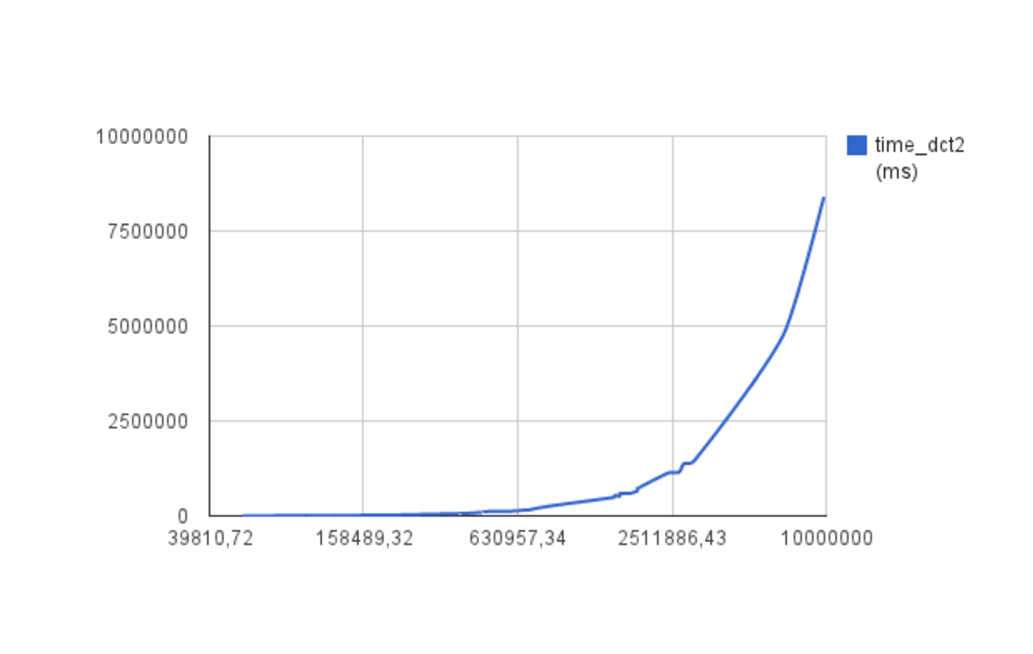
\includegraphics{grafico_dct2.eps}
\caption{Grafico dct2 implementata}
\end{figure}
\\\\
\begin{figure}[htbp]
\centering
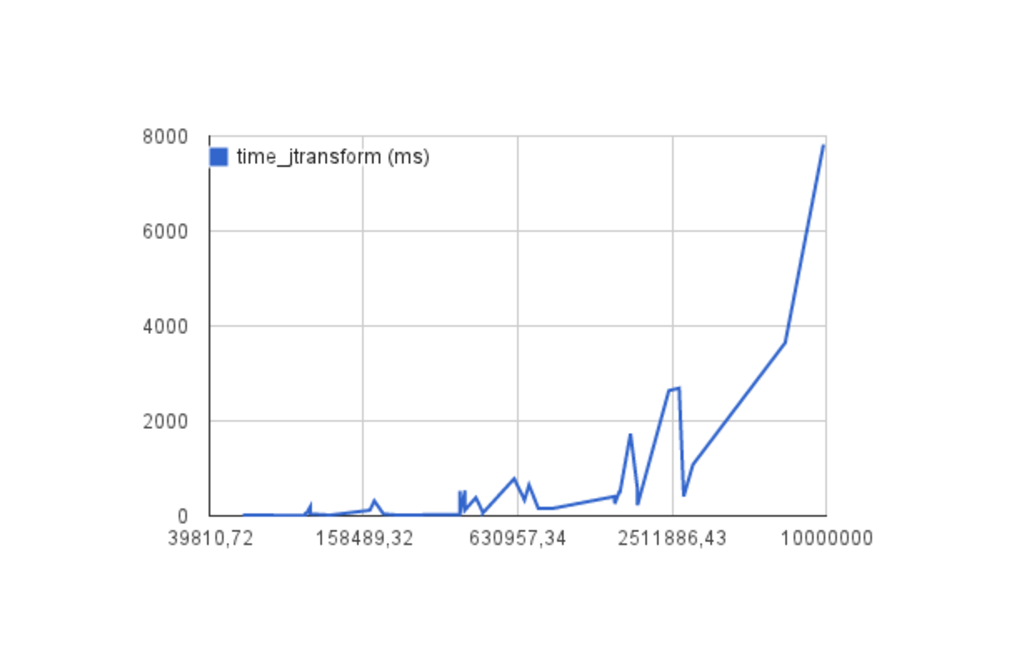
\includegraphics{grafico_jtransform.eps}
\caption{Grafico dct2 FAST}
\end{figure}
\\\\
\begin{table}[!h]
\begin{tabular}{|l|r|r|r|r|}
\hline
Name & Time Dct2 (ms) & Time Jt. (ms) & width (px) & height (px) \\ 
\hline
scaled/scaled/scaled/artificial.bmp & 7942 & 193 & 384 & 256 \\ 
scaled/scaled/scaled/big\_building.bmp & 127478 & 783 & 902 & 677 \\ 
scaled/scaled/scaled/big\_tree.bmp & 81907 & 383 & 761 & 569 \\ 
scaled/scaled/scaled/bridge.bmp & 19125 & 316 & 344 & 507 \\ 
scaled/scaled/scaled/cathedral.bmp & 7479 & 79 & 250 & 376 \\ 
scaled/scaled/scaled/deer.bmp & 18021 & 118 & 506 & 331 \\ 
scaled/scaled/scaled/fireworks.bmp & 10058 & 19 & 392 & 294 \\ 
scaled/scaled/scaled/flower\_foveon.bmp & 3284 & 18 & 284 & 189 \\ 
scaled/scaled/scaled/hdr.bmp & 7875 & 40 & 384 & 256 \\ 
scaled/scaled/scaled/leaves\_iso\_200.bmp & 7438 & 10 & 376 & 250 \\ 
scaled/scaled/scaled/leaves\_iso\_1600.bmp & 7551 & 10 & 376 & 250 \\ 
scaled/scaled/scaled/nightshot\_iso\_100.bmp & 10080 & 33 & 392 & 294 \\ 
scaled/scaled/scaled/nightshot\_iso\_1600.bmp & 10245 & 10 & 392 & 294 \\ 
scaled/scaled/scaled/spider\_web.bmp & 22486 & 38 & 532 & 356 \\ 
scaled/scaled/scaled/zone\_plate.bmp & 7588 & 8 & 375 & 250 \\ 
scaled/scaled/artificial.bmp & 66245 & 534 & 768 & 512 \\ 
scaled/scaled/big\_building.bmp & 1135163 & 2639 & 1804 & 1354 \\ 
scaled/scaled/big\_tree.bmp & 597656 & 1731 & 1522 & 1138 \\ 
scaled/scaled/bridge.bmp & 157433 & 650 & 688 & 1014 \\ 
scaled/scaled/cathedral.bmp & 60869 & 118 & 500 & 752 \\ 
scaled/scaled/deer.bmp & 151674 & 335 & 1012 & 662 \\ 
scaled/scaled/fireworks.bmp & 82743 & 82 & 784 & 588 \\ 
scaled/scaled/flower\_foveon.bmp & 25788 & 17 & 568 & 378 \\ 
scaled/scaled/hdr.bmp & 63813 & 125 & 768 & 512 \\ 
scaled/scaled/leaves\_iso\_200.bmp & 60658 & 527 & 752 & 500 \\ 
scaled/scaled/leaves\_iso\_1600.bmp & 61871 & 68 & 752 & 500 \\ 
scaled/scaled/nightshot\_iso\_100.bmp & 82330 & 111 & 784 & 588 \\ 
scaled/scaled/nightshot\_iso\_1600.bmp & 111011 & 59 & 784 & 588 \\ 
scaled/scaled/spider\_web.bmp & 207638 & 161 & 1064 & 712 \\ 
scaled/scaled/zone\_plate.bmp & 60285 & 29 & 750 & 500 \\ 
scaled/artificial.bmp & 518198 & 535 & 1536 & 1024 \\ 
scaled/big\_building.bmp & 8364020 & 7823 & 3608 & 2708 \\ 
scaled/big\_tree.bmp & 4872149 & 3647 & 3044 & 2276 \\ 
scaled/bridge.bmp & 1369571 & 411 & 1376 & 2028 \\ 
scaled/cathedral.bmp & 540372 & 267 & 1000 & 1504 \\ 
scaled/deer.bmp & 1151979 & 2690 & 2024 & 1324 \\ 
scaled/fireworks.bmp & 658911 & 568 & 1568 & 1176 \\ 
scaled/flower\_foveon.bmp & 267050 & 155 & 1136 & 756 \\ 
scaled/hdr.bmp & 585721 & 469 & 1536 & 1024 \\ 
scaled/leaves\_iso\_200.bmp & 525412 & 335 & 1504 & 1000 \\ 
scaled/leaves\_iso\_1600.bmp & 540518 & 256 & 1504 & 1000 \\ 
scaled/nightshot\_iso\_100.bmp & 727666 & 227 & 1568 & 1176 \\ 
scaled/nightshot\_iso\_1600.bmp & 720260 & 225 & 1568 & 1176 \\ 
scaled/spider\_web.bmp & 1416648 & 1079 & 2128 & 1424 \\ 
scaled/zone\_plate.bmp & 491263 & 408 & 1500 & 1000 \\
\hline
\end{tabular}
\end{table}

\subsection{Filtro delle frequenze}
La DCT \`e perfettamente reversibile e non perdiamo definizione dell'immagine. \\
Nel caso in cui vogliamo tagliare un certo numero di frequenze definiamo DCT(M\%), dove che sia per altezza che larghezza prendiamo $\frac{M}{100} \cdot N$ valori, dove N sono i valori totali. \\
Nelle figure sottostanti vediamo nelle prime quattro, il caso in cui tagliamo le frequenze con la mia implementazione e nelle quattro foto successive il filtraggio con l'implementazione FAST (Jtransforms). \\
Come vediamo JTransforms non \`e infallibile, in alcuni casi, se si tagliano certe frequenze, non riesce pi\`u a ricostruire l'immagine, questo \`e causato dal fatto che sono pi\`u thread che cercano di collaborare, si ricade su un problema di threads ed \`e un baco noto. \\
\begin{figure}[htbp]
\centering
\subfigure[Immagine originale]
{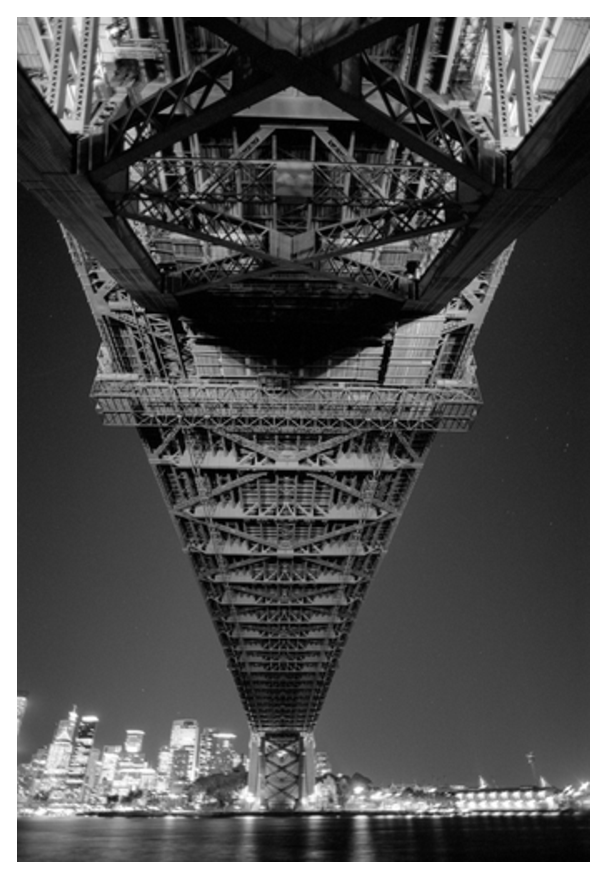
\includegraphics[width=8cm]{bridge.eps}}
\hspace{5mm}
\subfigure[DCT(50\%)]
{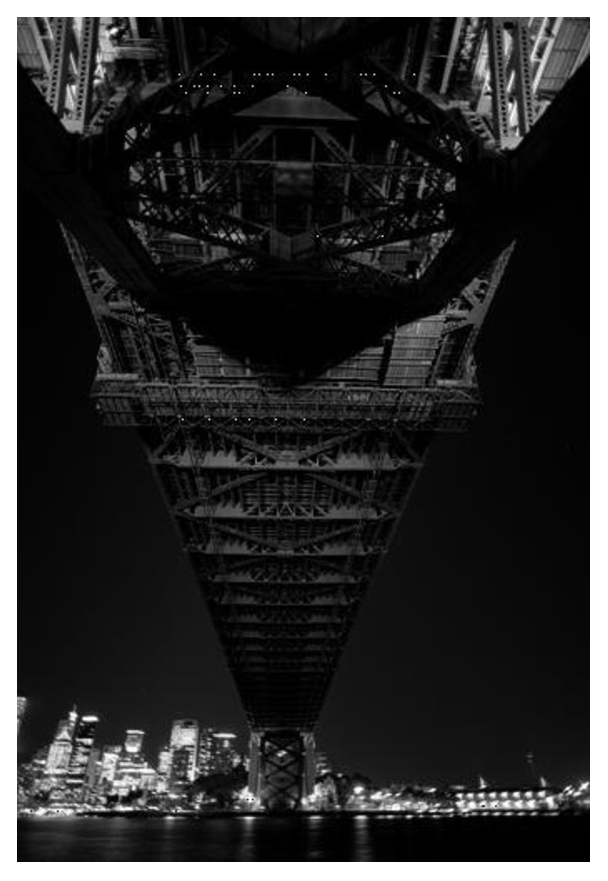
\includegraphics[width=8cm]{bridge-0500.eps}}
\subfigure[DCT(10\%)]
{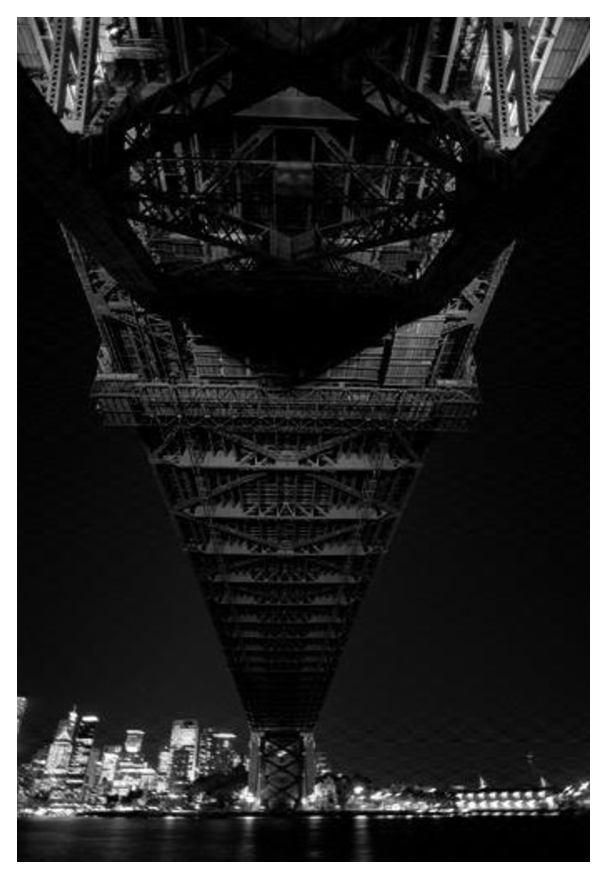
\includegraphics[width=8cm]{bridge-0100.eps}}
\hspace{5mm}
\subfigure[DCT(1\%)]
{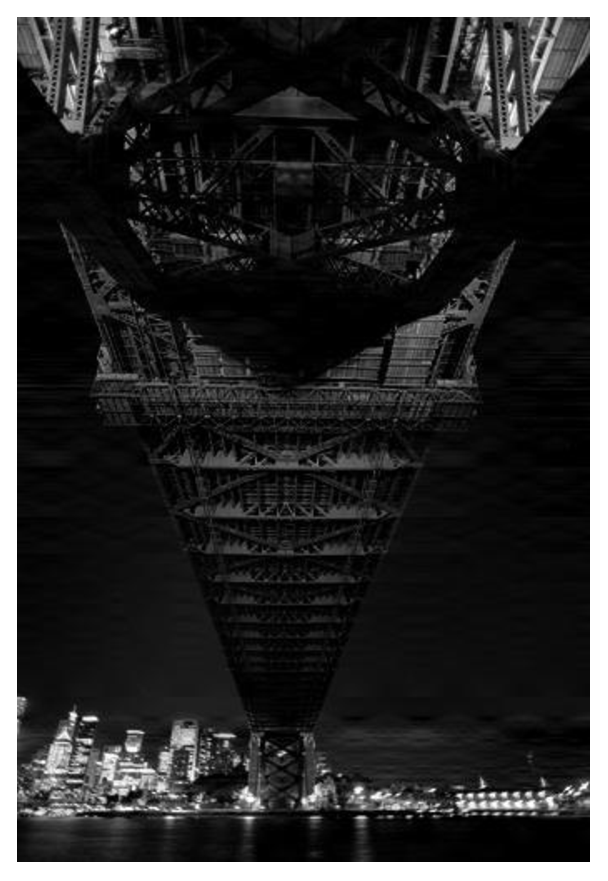
\includegraphics[width=8cm]{bridge-0010.eps}}
\end{figure} \\
\begin{figure}[htbp]
\centering
\subfigure[Immagine originale]
{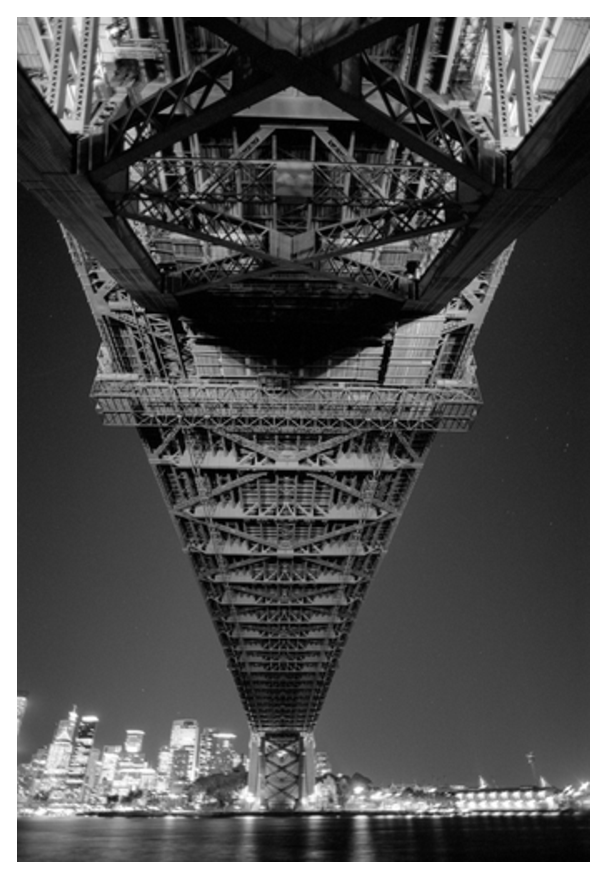
\includegraphics[width=8cm]{bridge.eps}}
\hspace{5mm}
\subfigure[FAST DCT(50\%)]
{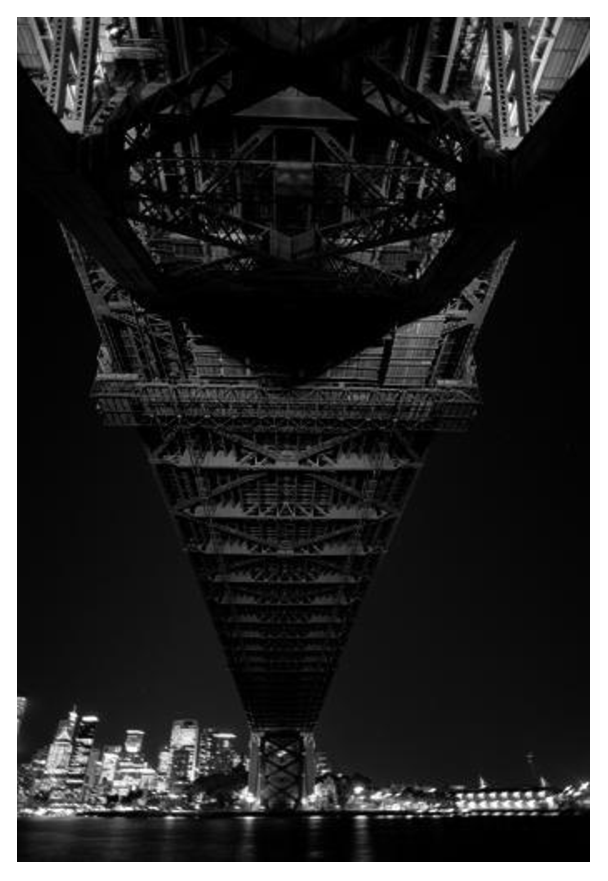
\includegraphics[width=8cm]{bridge-0500-fast.eps}}
\subfigure[FAST DCT(10\%)]
{
\includegraphics[width=8cm]{bridge-0100-fast.eps}}
\hspace{5mm}
\subfigure[FAST DCT(1\%)]
{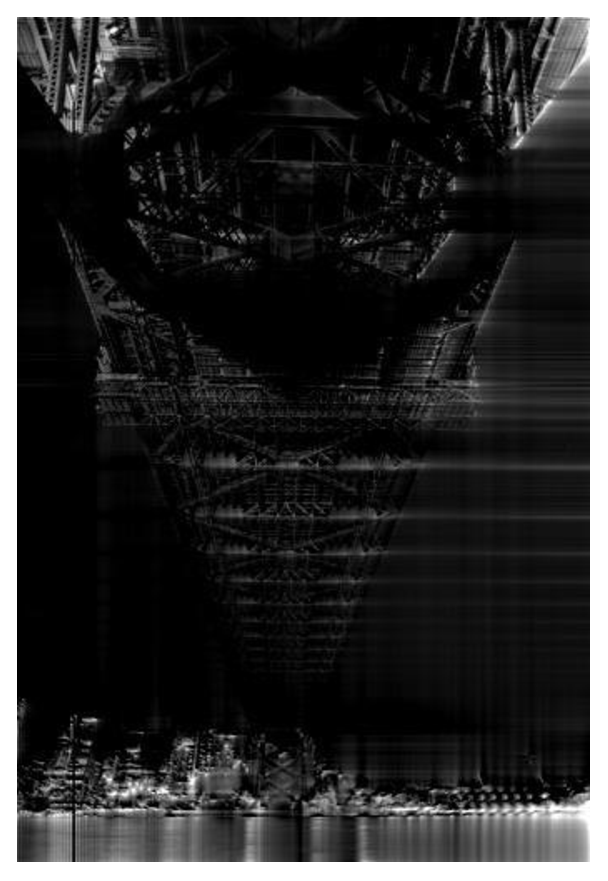
\includegraphics[width=8cm]{bridge-0010-fast.eps}}
\end{figure} \\
\end{document}
